% presentation/main.tex
% presentation/preamble.tex
\documentclass[aspectratio=169,11pt]{beamer}

\usetheme{metropolis}

\usepackage[french]{babel}
\usepackage[T1]{fontenc}
\usepackage{amsmath,amssymb}
\usepackage{graphicx}
\usepackage{xcolor}
\usepackage{booktabs} 
\usepackage{tikz} 

% ==============================================================================
% PALETTE DE COULEURS PREMIUM (Style Infographie Minimaliste)
% ==============================================================================
\definecolor{PremiumDark}{RGB}{45,40,35}     % Un brun-noir très profond pour le texte et titres (lisibilité 100%)
\definecolor{SubtleTaupe}{RGB}{115,100,85}   % Un taupe élégant pour la structure secondaire
\definecolor{Cream}{RGB}{253,251,247}        % Fond crème doux, haut de gamme, qui repose les yeux
\definecolor{LuxuryGold}{RGB}{180,145,90}    % Or brossé pour les alertes, barres et puces
\definecolor{LightCard}{RGB}{245,240,230}    % Couleur de fond pour les blocs/boîtes de texte

% ==============================================================================
% CONFIGURATION DES COULEURS DE BASE
% ==============================================================================
\setbeamercolor{background canvas}{bg=Cream}
\setbeamercolor{normal text}{fg=PremiumDark}
\setbeamercolor{title}{fg=PremiumDark}
\setbeamercolor{subtitle}{fg=SubtleTaupe}
\setbeamercolor{frametitle}{fg=PremiumDark}
\setbeamercolor{structure}{fg=PremiumDark}
\setbeamercolor{alerted text}{fg=LuxuryGold}

% ==============================================================================
% DESIGN DU PIED DE PAGE (Nettoyé et Ultra-Clair)
% ==============================================================================
\metroset{progressbar=foot} 
\setbeamercolor{progress bar}{fg=LuxuryGold, bg=LightCard} % Barre fine Or sur fond discret

% Le texte du bas écrit en gris-brun fin directement sur le fond Crème
\setbeamercolor{footline}{fg=SubtleTaupe, bg=Cream} 
\setbeamercolor{page number in head/foot}{fg=SubtleTaupe}

% ==============================================================================
% CORRECTION CRITIQUE : Suppression des pages sombres de Metropolis
% ==============================================================================
% On force Metropolis à faire des pages de garde et de sections CLAIRES. 
% Plus aucun risque de texte noir caché sur fond marron !
\setbeamercolor{palette primary}{fg=PremiumDark, bg=Cream}

% ==============================================================================
% INFOGRAPHIE : Structure visuelle des Diapositives
% ==============================================================================
\setbeamertemplate{navigation symbols}{}

% Ligne de séparation or brossé sous le titre de chaque slide
\setbeamertemplate{frametitle}{%
    \begin{beamercolorbox}[wd=\paperwidth,ht=4ex,dp=1.5ex,leftskip=0.5cm]{frametitle}
        \usebeamerfont{frametitle}\insertframetitle
    \end{beamercolorbox}%
    \vspace{-0.1cm}
    {\color{LuxuryGold}\hrule height 0.8pt} 
    \vspace{0.2cm}
}

% Blocs Modernes style "Cards / Encadrés épurés"
\setbeamertemplate{blocks}[rounded][shadow=false]
\setbeamercolor{block title}{bg=SubtleTaupe, fg=Cream}
\setbeamercolor{block body}{bg=LightCard, fg=PremiumDark}

\setbeamercolor{block title alerted}{bg=LuxuryGold, fg=Cream}
\setbeamercolor{block body alerted}{bg=LuxuryGold!10, fg=PremiumDark}

% Puces d'infographie épurées
\setbeamertemplate{itemize item}{\color{LuxuryGold}$\blacktriangleright$}
\setbeamertemplate{itemize subitem}{\color{SubtleTaupe}$\bullet$}

% Typographie Mathématique Professionnelle
\usefonttheme{professionalfonts}

\newcommand{\R}{\mathbb{R}}
\newcommand{\E}{\mathbb{E}}
\DeclareMathOperator*{\argmax}{arg\,max}

\title{Estimation dans un problème inverse linéaire à variables cachées}
\subtitle{Vraisemblance, Algorithme EM et Analyse de l'Erreur}
\author{Arthur Conche \and Abdel Niang}
\institute{Université Paris Cité \\ M1 Mathématiques, Modélisation et Apprentissage Statistique}
\date{Année Universitaire 2025-2026}

\begin{document}

% Slide de Titre
% presentation/slides/01_title.tex
{
\setbeamercolor{background canvas}{bg=DarkBeige}
\setbeamercolor{normal text}{fg=Cream}
\setbeamercolor{title}{fg=Cream}
\setbeamercolor{subtitle}{fg=SoftGold}
\setbeamercolor{author}{fg=Cream}
\setbeamercolor{date}{fg=Cream}
\setbeamercolor{institute}{fg=Cream}
\setbeamercolor{progress bar}{fg=SoftGold}
\begin{frame}[plain]
    \titlepage
\end{frame}
}

% Partie 1 : Chapitre 1 - Mise en place du problème
\section{Mise en place du problème et Modélisation}
% presentation/slides/02_cryo.tex
\begin{frame}{Le Contexte Physique : La Cryo-EM}
    \begin{columns}[c]
        \begin{column}{0.5\textwidth}
            \large\textbf{Principe de la Cryo-Microscopie Électronique}\\[0.3cm]
            \normalsize
            \begin{itemize}
                \item Des milliers de macromolécules figées dans de la glace amorphe.
                \item Le faisceau d'électrons capture des \alert{projections 2D}.
                \item \textbf{Le problème majeur :} L'orientation tridimensionnelle sous laquelle chaque photo est prise est \textbf{inconnue}.
                \item Le signal observé est noyé dans un niveau de bruit extrême ($\text{RSB} \ll 1$).
            \end{itemize}
        \end{column}
        \begin{column}{0.5\textwidth}
            \centering
            % Remplacer par 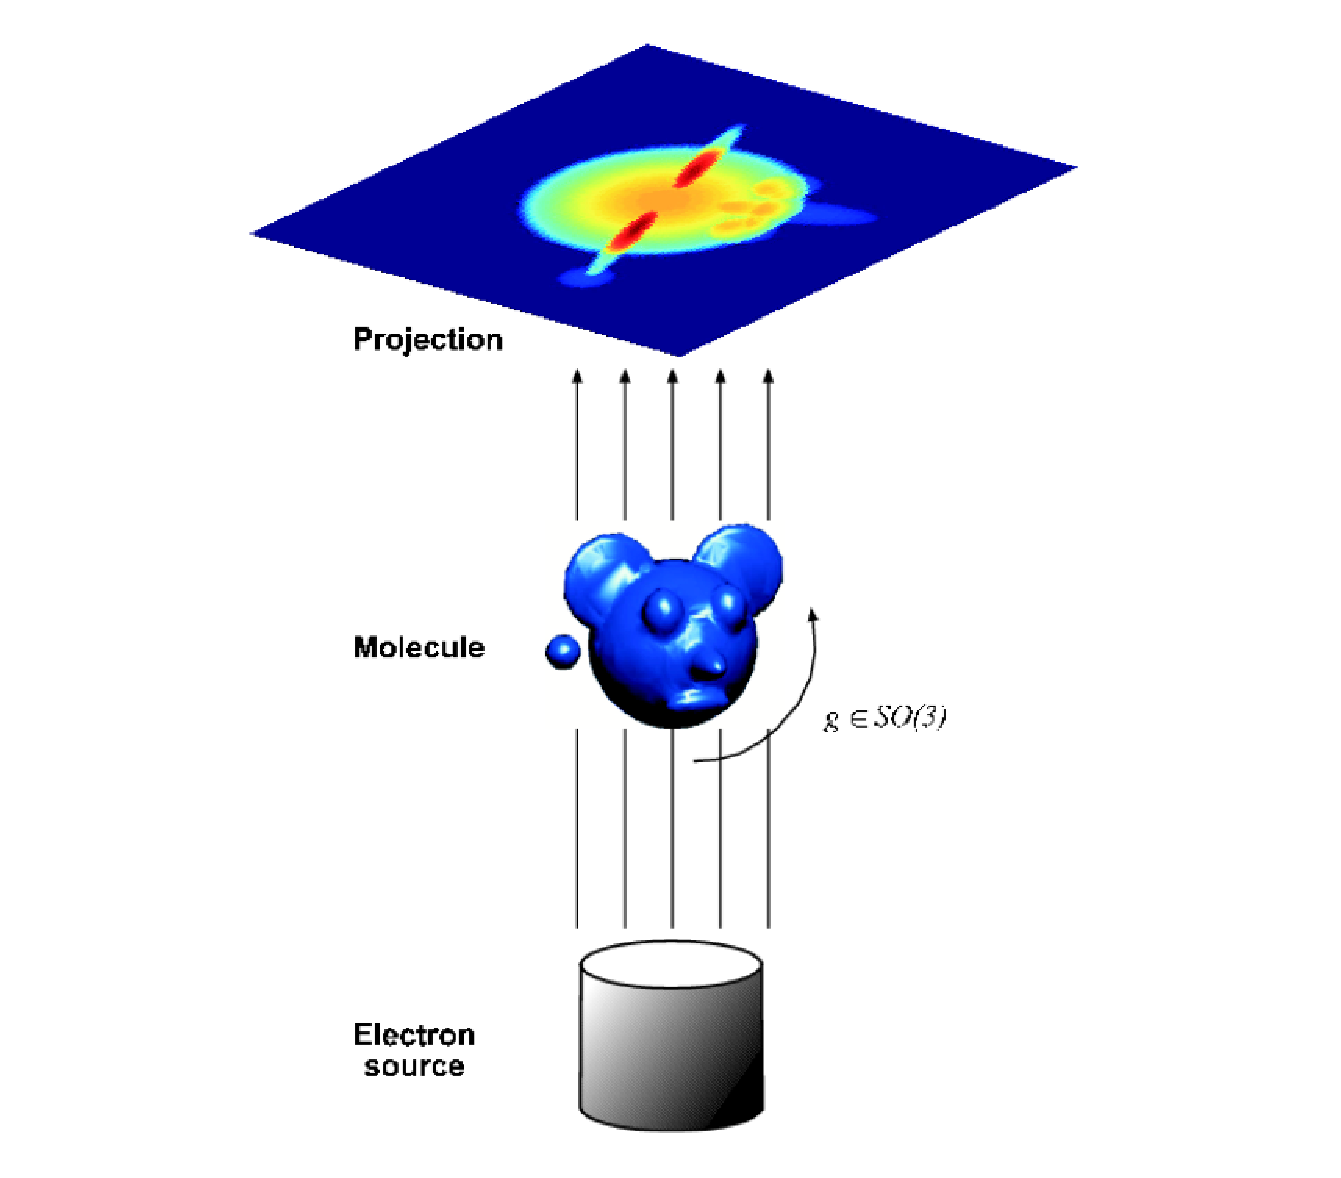
\includegraphics[width=0.9\textwidth]{figures/cryo-Singer.pdf} en local
            \framebox{\begin{minipage}{0.8\textwidth}\centering\vspace{1.5cm}\textcolor{DarkBeige}{\textbf{[ figures/cryo-Singer.pdf ]}}\\\small Schéma Cryo-EM / Projections\vspace{1.5cm}\end{minipage}}
        \end{column}
    \end{columns}
\end{frame}
% presentation/slides/03_modele.tex
\begin{frame}{Le Modèle Mathématique Général}
    Pour chaque observation $i \in \{1, \dots, n\}$, on formule l'équation :
    
    \begin{center}
        \Large \alert{$Y_i = A_{Z_i}\theta + \sigma E_i$}
    \end{center}
    
    \vspace{0.4cm}
    \begin{itemize}
        \item $\mathbf{\theta \in E}$ : Le paramètre ou signal d'intérêt \textbf{inconnu} à estimer ($\dim E = d$).
        \item $\mathbf{Z_i \in \mathcal{Z}}$ : La \textbf{variable cachée} (la transformation géométrique subie par l'objet), supposée i.i.d. selon une loi connue $f_Z$.
        \item $\mathbf{A_{Z_i}}$ : L'opérateur linéaire modélisant la transformation (translation, rotation, projection).
        \item $\mathbf{E_i \sim \mathcal{N}(0, \text{Id}_p)}$ : Un bruit blanc gaussien i.i.d., indépendant de $Z_i$.
        \item $\mathbf{\sigma > 0}$ : Le niveau de bruit de l'appareil de mesure.
    \end{itemize}
\end{frame}
% presentation/slides/04_cas1.tex
\begin{frame}{Le Cas d'Application Linéaire 1D}
    \begin{columns}[c]
        \begin{column}{0.55\textwidth}
            \textbf{Modèle Jouet : Décalages circulaires (Translations sur le Tore)}
            \begin{itemize}
                \item $\theta$ est un signal périodique modélisé dans la base de Fourier.
                \item Les variables cachées $Z_i$ représentent des translations uniformes sur la grille discretisée.
                \item L'opérateur $A_{Z_i}$ applique un déphasage en fréquences.
            \end{itemize}
            \vspace{0.2cm}
            \alert{\textbf{Piège Statistique :}} La moyenne empirique brute $\frac{1}{n}\sum Y_i$ converge vers un signal plat. L'information de phase s'efface !
        \end{column}
        \begin{column}{0.45\textwidth}
            \centering
            % Remplacer par 
\includegraphics[width=0.9\textwidth]{figures/signaux_1D.pdf}
            \framebox{\begin{minipage}{0.9\textwidth}\centering\vspace{1.2cm}\textcolor{DarkBeige}{\textbf{[ figures/signaux_1D.pdf ]}}\\\small Signaux simulés translatés\vspace{1.2cm}\end{minipage}}
        \end{column}
    \end{columns}
\end{frame}

% Partie 2 : Chapitre 4 - Vraisemblance & Algorithmes
\section{Méthodes d'Estimation Numérique}
% presentation/slides/05_vraisemblance.tex
\begin{frame}{Le Défi de la Log-Vraisemblance Marginale}
    Puisque les variables $Z_i$ sont manquantes, on doit intégrer (marginaliser) la densité conjointe :
    
    $$l_n(\theta) = \sum_{i=1}^n \log \left( \int_{\mathcal{Z}} f_Y(Y_i | Z=z, \theta) f_Z(z) d\mu(z) \right)$$
    
    \vspace{0.2cm}
    \textbf{Une structure non linéaire complexe (Log-Sum-Exp) :}
    \begin{itemize}
        \item $l_n(\theta)$ \alert{\textbf{n'est plus concave}}, invalidant une optimisation exacte globale directe.
        \item Présence de multiples \textbf{maximums locaux} (pièges pour les algorithmes).
        \item \textbf{Défaut d'identifiabilité :} Le problème est invariant à une translation globale près. On doit introduire une \textbf{distance quotient d'orbite} :
        $$d_{\text{orbite}}(\theta, \theta^*) = \min_{z \in \mathcal{Z}} \| \theta - A_z \theta^* \|$$
    \end{itemize}
\end{frame}
% presentation/slides/06_gradient_em.tex
\begin{frame}{Descente de Gradient Directe vs Approche EM}
    Pour maximiser $l_n(\theta)$, deux choix algorithmiques s'opposent :
    
    \vspace{0.4cm}
    \begin{columns}[t]
        \begin{column}{0.48\textwidth}
            \setbeamercolor{block title}{bg=DarkBeige,fg=Cream}
            \begin{block}{\textbf{Descente de Gradient Directe}}
                \small
                \begin{itemize}
                    \item Calcul direct du gradient de la log-vraisemblance marginale.
                    \item Fait intervenir les poids a posteriori $w_{i,z}(\theta)$.
                    \item Sensible au choix du pas (Règle d'Armijo nécessaire).
                    \item \alert{Nécessite des stratégies multi-départs} pour échapper aux extrema locaux.
                \end{itemize}
            \end{block}
        \end{column}
        
        \begin{column}{0.48\textwidth}
            \setbeamercolor{block title}{bg=SoftGold,fg=Cream}
            \begin{block}{\textbf{Algorithme EM}}
                \small
                \begin{itemize}
                    \item Maximise une borne inférieure via les \textbf{données complètes} $(Y, Z)$.
                    \item Propriété de \textbf{croissance monotone} de la vraisemblance à chaque étape.
                    \item Découple la complexité : l'étape d'inversion redevient quadratique et linéaire.
                \end{itemize}
            \end{block}
        \end{column}
    \end{columns}
\end{frame}
% presentation/slides/07_em.tex
\begin{frame}{Les Deux Étapes Clés de l'Algorithme EM}
    À l'itération $k$, on calcule l'estimation récursive $\theta^{(k+1)}$ :

    \textbf{Étape E (Espérance) :} Calcul des probabilités a posteriori (\textit{poids}) pour chaque échantillon $i$ et transformation $z$ :
    $$w_{i,z}(\theta^{(k)}) = \frac{f_Z(z) \exp\left(-\frac{\|Y_i - A_z\theta^{(k)}\|^2}{2\sigma^2}\right)}{\int_{\mathcal{Z}} f_Z(z') \exp\left(-\frac{\|Y_i - A_{z'}\theta^{(k)}\|^2}{2\sigma^2}\right) d\mu(z')}$$

    \textbf{Étape M (Maximisation) :} Résolution d'un point fixe sous forme de système linéaire :
    $$\left( \sum_{i=1}^n \int_{\mathcal{Z}} w_{i,z}(\theta^{(k)}) A_z^\top A_z d\mu(z) \right) \alert{\theta^{(k+1)}} = \sum_{i=1}^n \int_{\mathcal{Z}} w_{i,z}(\theta^{(k)}) A_z^\top Y_i d\mu(z)$$
    L'étape M est un problème \textbf{quadratique convexe}, trivial à résoudre numériquement.
\end{frame}

% Partie 3 : Chapitre 6 - Régularisation
\section{Analyse Spectrale et Régularisation}
% presentation/slides/08_regularisation.tex
\begin{frame}{Le Problème Inverse Mal Posé en Dimension Supérieure}
    \begin{columns}[c]
        \begin{column}{0.55\textwidth}
            \large\textbf{La Rupture Géométrique (Cas 2D / Radon)}\\[0.2cm]
            \normalsize
            \begin{itemize}
                \item En projection 2D, l'opérateur $A_z$ lisse intensément le signal.
                \item Le spectre de l'opérateur décroît en \alert{$|\xi|^{-1}$} (Théorème de la tranche de Fourier).
                \item La matrice de l'étape M devient \textbf{très mal conditionnée} (valeurs propres proches de 0).
                \item \textbf{Conséquence :} Le bruit de mesure $\sigma E_i$ est multiplié par $1/\lambda_k$ et explose en haute fréquence.
            \end{itemize}
        \end{column}
        \begin{column}{0.45\textwidth}
            \centering
            % Remplacer par \includegraphics[width=0.9\textwidth]{figures/"spectre_ATA.pdf"}
            \framebox{\begin{minipage}{0.9\textwidth}\centering\vspace{1.2cm}\textcolor{DarkBeige}{\textbf{[ figures/spectre_ATA.pdf ]}}\\\small Évanouissement des valeurs propres\vspace{1.2cm}\end{minipage}}
        \end{column}
    \end{columns}
\end{frame}
% presentation/slides/09_tikhonov.tex
\begin{frame}{Stratégies de Stabilisation : Tikhonov et Pénalités}
    Pour stabiliser le système, on modifie la fonction objectif en ajoutant une pénalité :
    
    \begin{center}
        \large $l_n^{\text{reg}}(\theta) = l_n(\theta) - \alert{\lambda \mathcal{R}(\theta)}$
    \end{center}
    
    \vspace{0.2cm}
    \begin{itemize}
        \item \textbf{Régularisation de Tikhonov ($L^2$) :} $\mathcal{R}(\theta) = \frac{1}{2}\|\theta\|^2_2$.
        \begin{itemize}
            \item Décale artificiellement les valeurs propres de la matrice : $\lambda_j \leftarrow \lambda_j + \lambda\sigma^2$.
            \item Empêche l'inversion de diviser par zéro, supprimant les oscillations hautes fréquences.
        \end{itemize}
        \item \textbf{Régularisation Lasso ($L^1$) :} $\mathcal{R}(\theta) = \|\theta\|_1 \implies$ Favorise des solutions \textbf{parcimonieuses} (creuses).
        \item \textbf{Variation Totale (TV) :} $\mathcal{R}(\theta) = \|\nabla \theta\|_1 \implies$ Préserve les contours et les zones homogènes (adapté au cas 2D).
    \end{itemize}
\end{frame}
% presentation/slides/10_resultats.tex
\begin{frame}{Observations Numériques et Analyse d'Erreur}
    \begin{columns}[c]
        \begin{column}{0.5\textwidth}
            \centering
            % Remplacer par 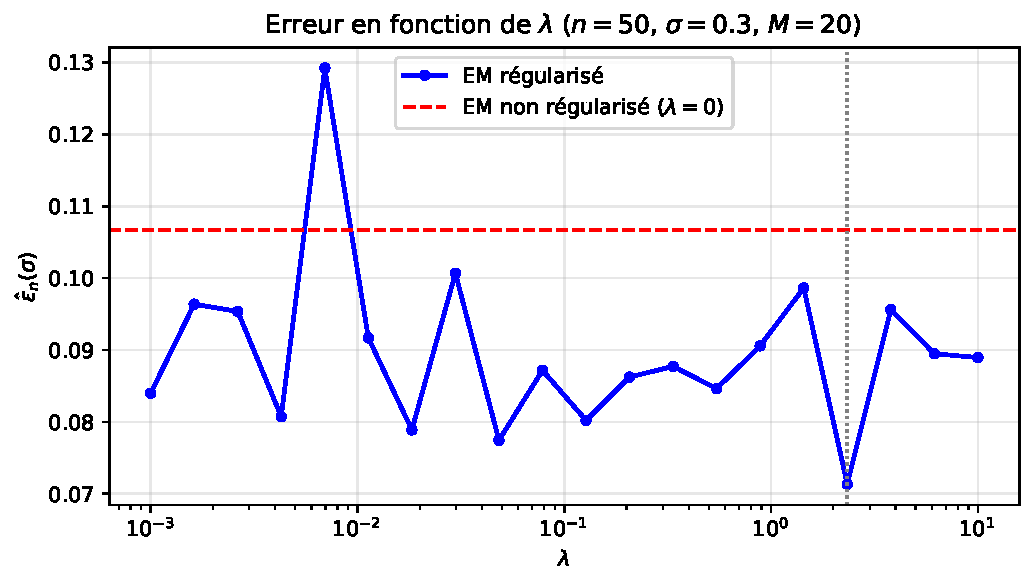
\includegraphics[width=0.85\textwidth]{figures/erreur_vs_lambda.pdf}
            \framebox{\begin{minipage}{0.85\textwidth}\centering\vspace{1.0cm}\textcolor{DarkBeige}{\textbf{[ erreur_vs_lambda.pdf ]}}\\\small Compromis biais-variance sur $\lambda$\vspace{1.0cm}\end{minipage}}
        \end{column}
        \begin{column}{0.5\textwidth}
            \centering
            % Remplacer par 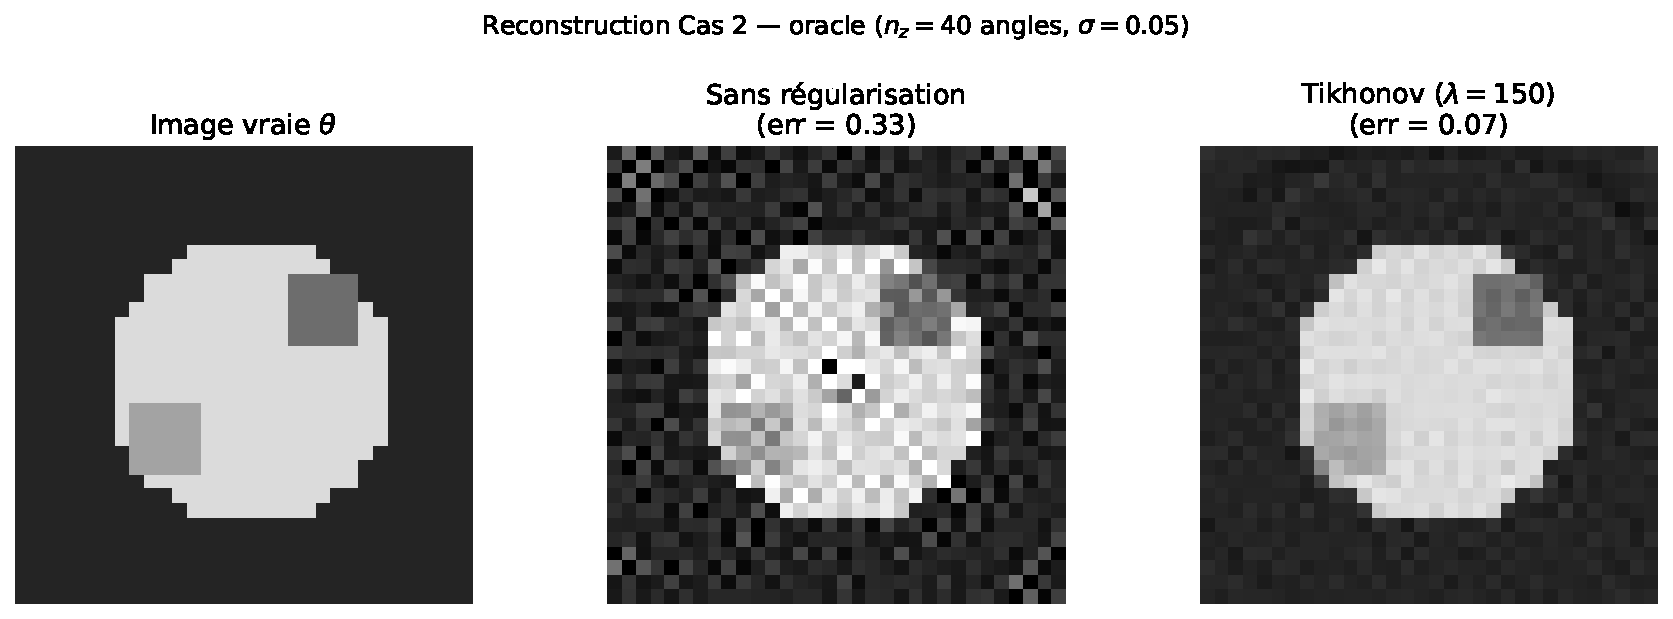
\includegraphics[width=0.85\textwidth]{figures/reconstruction_2d.pdf}
            \framebox{\begin{minipage}{0.85\textwidth}\centering\vspace{1.0cm}\textcolor{DarkBeige}{\textbf{[ reconstruction_2d.pdf ]}}\\\small Impact de la TV en 2D\vspace{1.0cm}\end{minipage}}
        \end{column}
    \end{columns}
    \vspace{0.3cm}
    \begin{center}
        \small \textbf{L'indispensable compromis :} Si $\lambda$ est trop faible, le bruit submerge l'image. Si $\lambda$ est trop fort, les détails structuraux fins s'estompent (biais élevé).
    \end{center}
\end{frame}

% Conclusion & Fin
% presentation/slides/11_conclusion.tex
\begin{frame}{Conclusion et Perspectives}
    \textbf{Trois enseignements fondamentaux :}
    \begin{enumerate}
        \item \textbf{Le coût statistique du masque :} L'absence géométrique d'information ($Z_i$ cachés) détruit la linéarité classique et introduit de la non-convexité via le profil \textit{log-sum-exp}.
        \item \textbf{La puissance découplée de l'EM :} L'algorithme EM s'avère optimal en pratique en reformulant l'étape M complexe en itérations de sous-problèmes convexes et linéaires stables.
        \item \textbf{Complémentarité Statistique-Régularisation :}} La quantité de données ($n \to \infty$) réduit l'erreur de variance, mais seule la pénalisation mathématique structurelle gère le caractère mal posé de la physique (Radon 2D).
    \end{enumerate}
    
    \vspace{0.2cm}
    \textbf{Ouverture :} Généralisation en 3D (espace des rotations non commutatif $SO(3)$) et traitement des hétérogénéités de distribution de $f_Z$.
\end{frame}
% presentation/slides/12_questions.tex
{
\setbeamercolor{background canvas}{bg=DarkBeige}
\setbeamercolor{normal text}{fg=Cream}
\setbeamercolor{frametitle}{fg=Cream}
\begin{frame}[plain]
    \centering
    \vspace{2cm}
    \Huge \textcolor{Cream}{\textbf{Merci pour votre attention}}
    
    \vspace{0.8cm}
    \large \textcolor{SoftGold}{\textbf{Place aux questions}}
    
    \vspace{1.5cm}
    \footnotesize \textcolor{Cream}{Estimation dans un problème inverse linéaire à variables cachées \\ Université Paris Cité - M1 Mathématiques}
\end{frame}
}

\end{document}